The previous chapter looked at persistent memory programming from the perspective of consistency models and programming interface.
While necessary to define correct program behavior, I did not consider actual implementations or what optimizations provide optimal performance.
This chapter considers two simple persistent programming patterns -- a persistent log/buffer and a persistent linked list.
While I will describe how the persistent memory consistency models of the previous chapters operate with each, the point is to highlight potential performance bottlenecks and necessary optimizations.
I do not yet consider actual programming models or hardware to provide these optimizations.

\section{Performance}
\label{sec:PMC_patterns:Performance}

In the previous chapter I made a number of statements regarding the performance of NVRAM without much explanation.
Here I describe how I expect NVRAM, the memory system, and the programming model to affect performance.
Later sections will use these assumptions to reason about data structure performance and imaging performance optimizations.

There are primarily two cases where persists may cause a thread to stall: ordering barriers and sync barriers.
Ordering barriers may operate by stalling at the barrier until all previous persists complete, obviously stalling the thread of execution.
More complex memory systems (such as BPFS) allow threads to continue executing ahead of persistent state, using a buffer to store persists (either in the cache or a memory buffer).
If these buffers become full threads will need to stall until room becomes available.
Therefore, persist throughput is the primary concern -- buffers allow threads to execute ahead of persistent state, but the average rate of persist must match the average rate of execution, otherwise stalls necessarily occur.

Persist throughput is primarily limited by the number of persist dependencies in an applications.
Memories typically allow high throughput so long as reads and writes may occur in parallel.
Persist dependencies reduce parallelism, requiring that some set of writes persist entirely before any dependent persists begin.
Since NVRAM cells may take up to microseconds to persists the longest dependence chain of persists may easily limit execution throughput and cause stalls.
Persistent memory consistency models stand to improve throughput and reduce stalls by relaxing persist ordering constraints and minimize the persist critical path.
The ultimate goal is to reduce persist critical path sufficiently that persist throughput exceeds execution throughput, providing the throughput of a DRAM system with the persistence of NVRAM.

Persistent memory applications also introduce stalls at sync barriers.
These are barriers used when interacting with the outside world (e.g., displaying something on-screen, communicating over the network).
Unless this external communication can be ordered with persists, allowing the thread to continue doing other useful work, the thread must stall for previous persists to complete, hurting throughput.
Additionally, end-to-end latency is important for many applications and tasks -- greater sync time (while persists drain/flush) leads to increased task latency.
Again, persist critical path determines sync latency; if all independent writes may persist in parallel the time to sync is determined by the longest chain of persists outstanding at the time sync is called.

The remainder of this chapter looks at two simple data structures, reasoning about durability while at the same time considering the persist critical path.
While some of the problems highlighted here can be circumvented by software techniques (e.g., only allowing a single thread to persist, using control flow to conditionally place epoch boundaries), this misses the point of persistent memory consistency -- to provide an easily programmable interface.
Rather, I assume the most straightforward and intuitive software design, investigating memory system optimizations.
However, I do not consider actual implementations.

\section{persistent buffer}
\label{sec:PMC_patterns:Buffer}

\begin{figure}
\centering
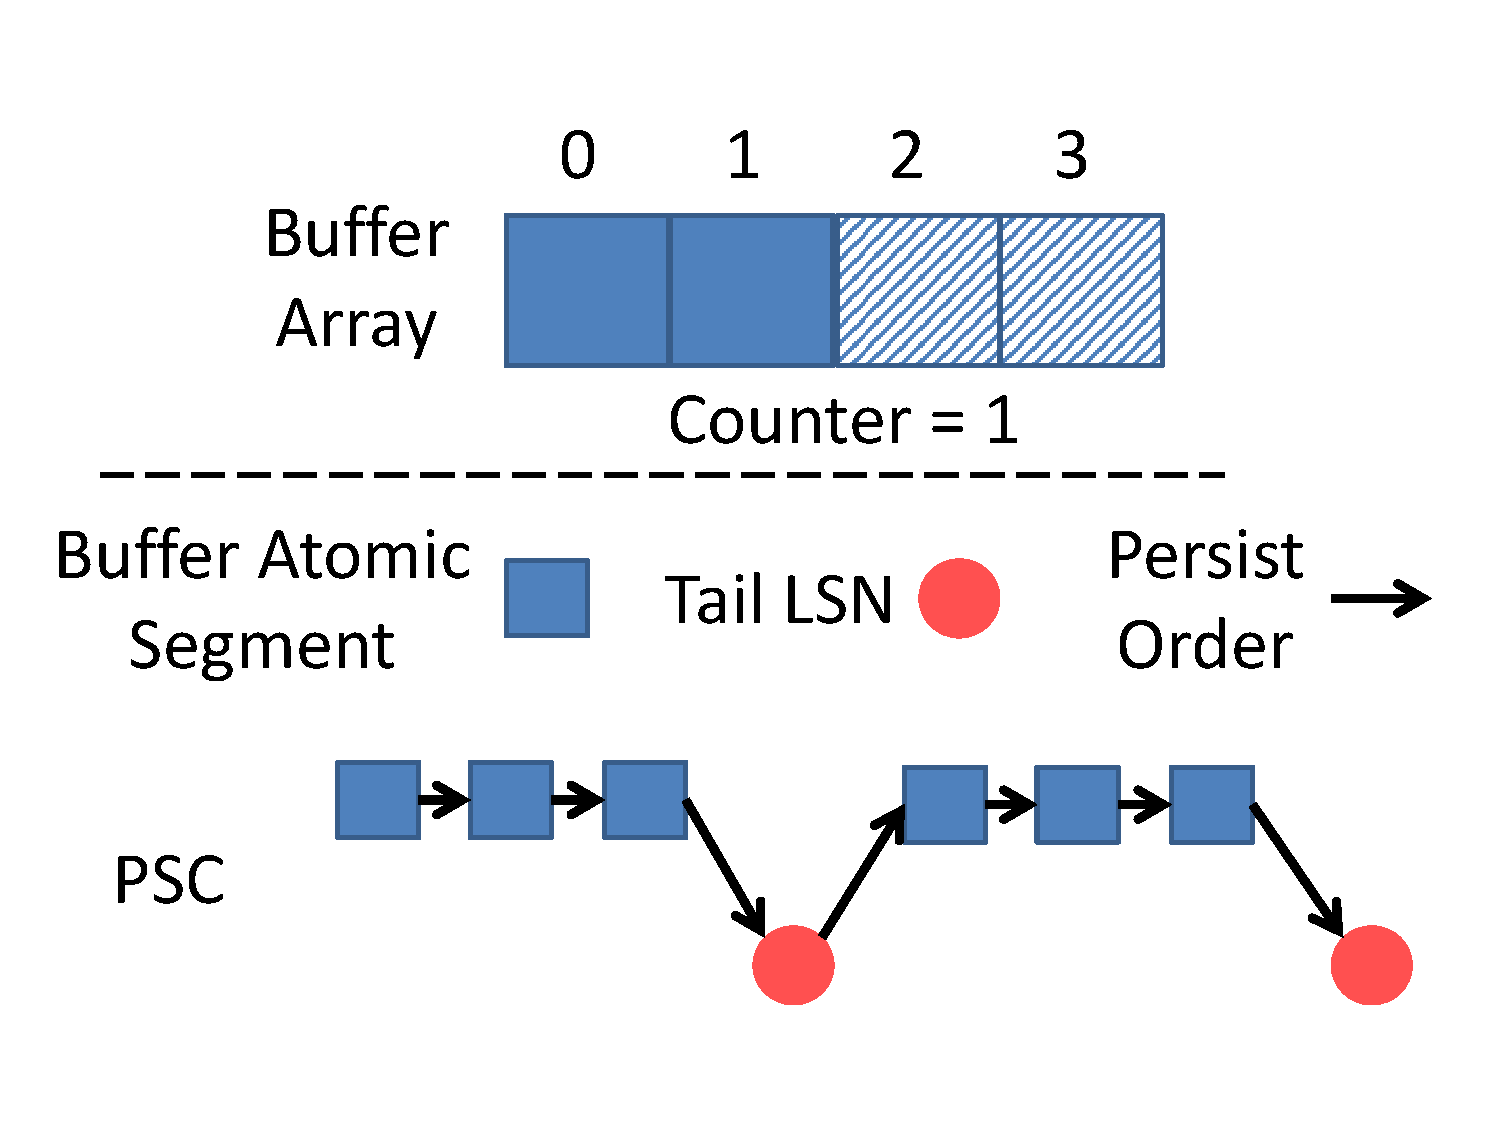
\includegraphics[width=\textwidth]{PMC_patterns/buffer.pdf}
\caption{Persistent buffer. The persistent buffer constists of a persistent array and counter (top).  The array holds persistent data.  The persistent counter marks the greatest persistent slot.  Persisting to the buffer under PSC places depdencies between writing buffer data and updating the counter, as well between persisting the counter and the next buffer persist, forming a chain (bottom).  This occurs both for single threaded and multithreaded use.}
\label{fig:buffer}
\end{figure}

\begin{figure}
\centering
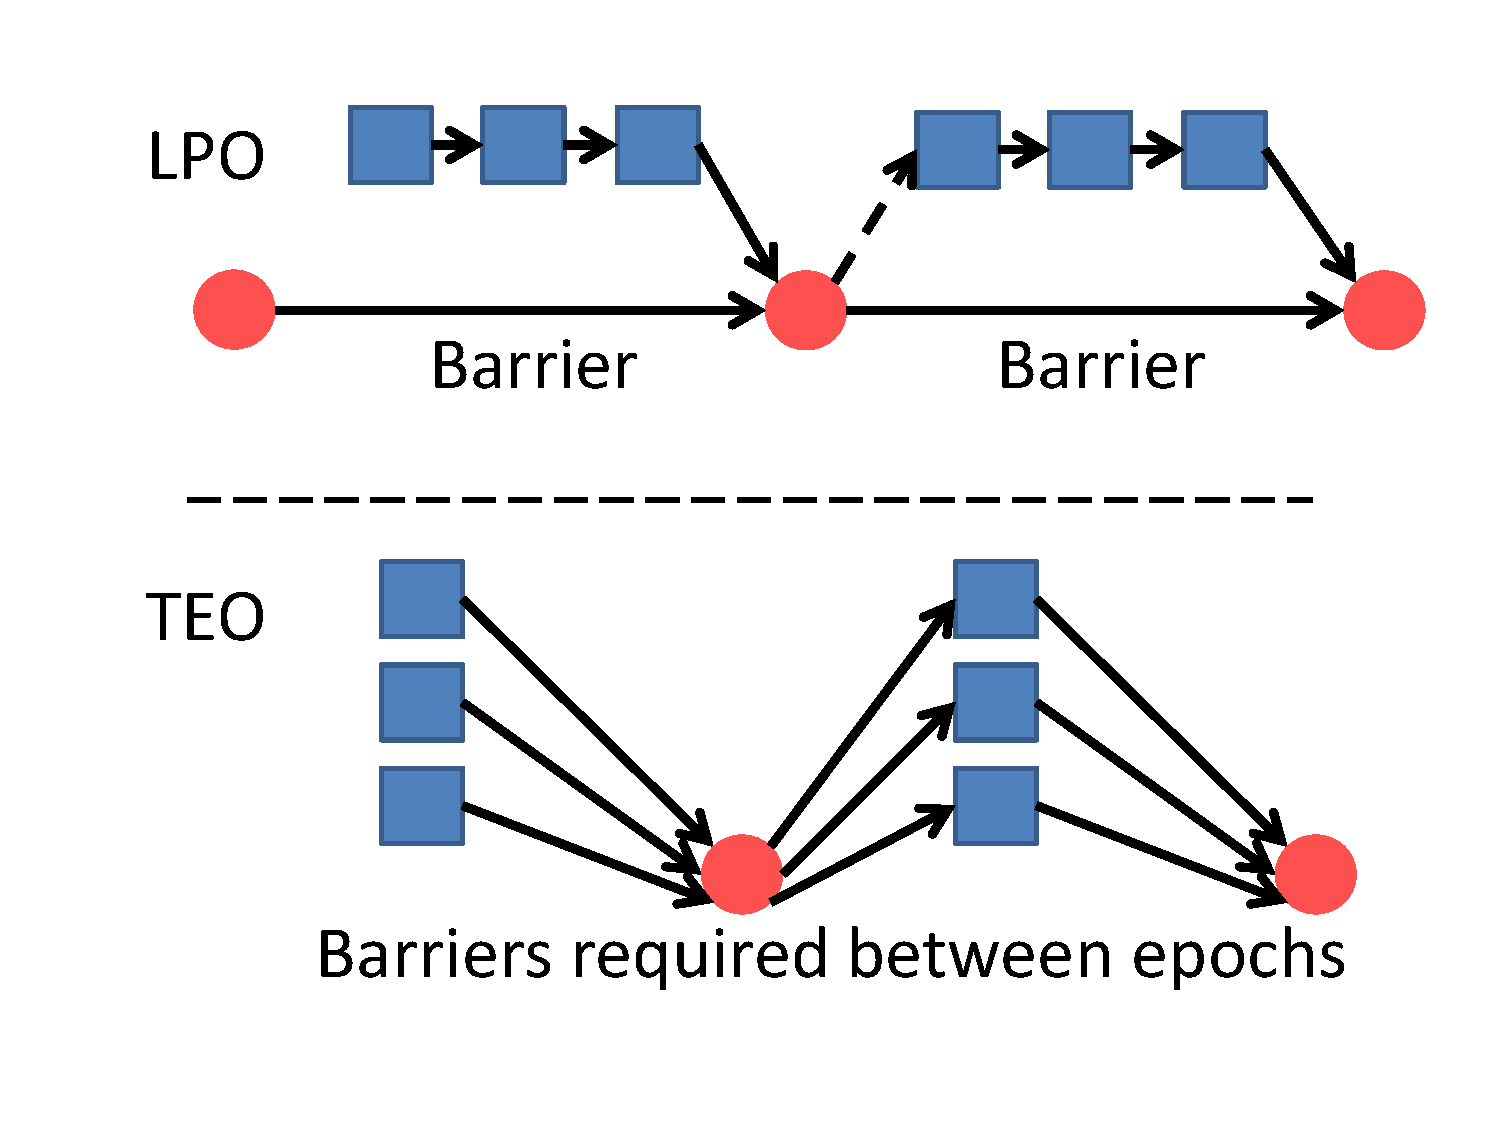
\includegraphics[width=\textwidth]{PMC_patterns/buffer_TEO_LPO.pdf}
\caption{Buffer execution under LPO and TEO.  LPO (top) removes persist dependencies between persisting the counter value and subsequent buffer persists.  Such dependencies still remain when adjacent buffer inserts are from the same thread.  Atomic persist segments within each buffer persist serialize.  TEO (bottom) allows buffer data to persist in parallel.  Buffer data necessarily persists before counter data for correctness, but counter values additionally persist before subsequent buffer persists, even from remote threads.}
\label{figure::buffer_TEO_LPO}
\end{figure}

\begin{figure}
\centering
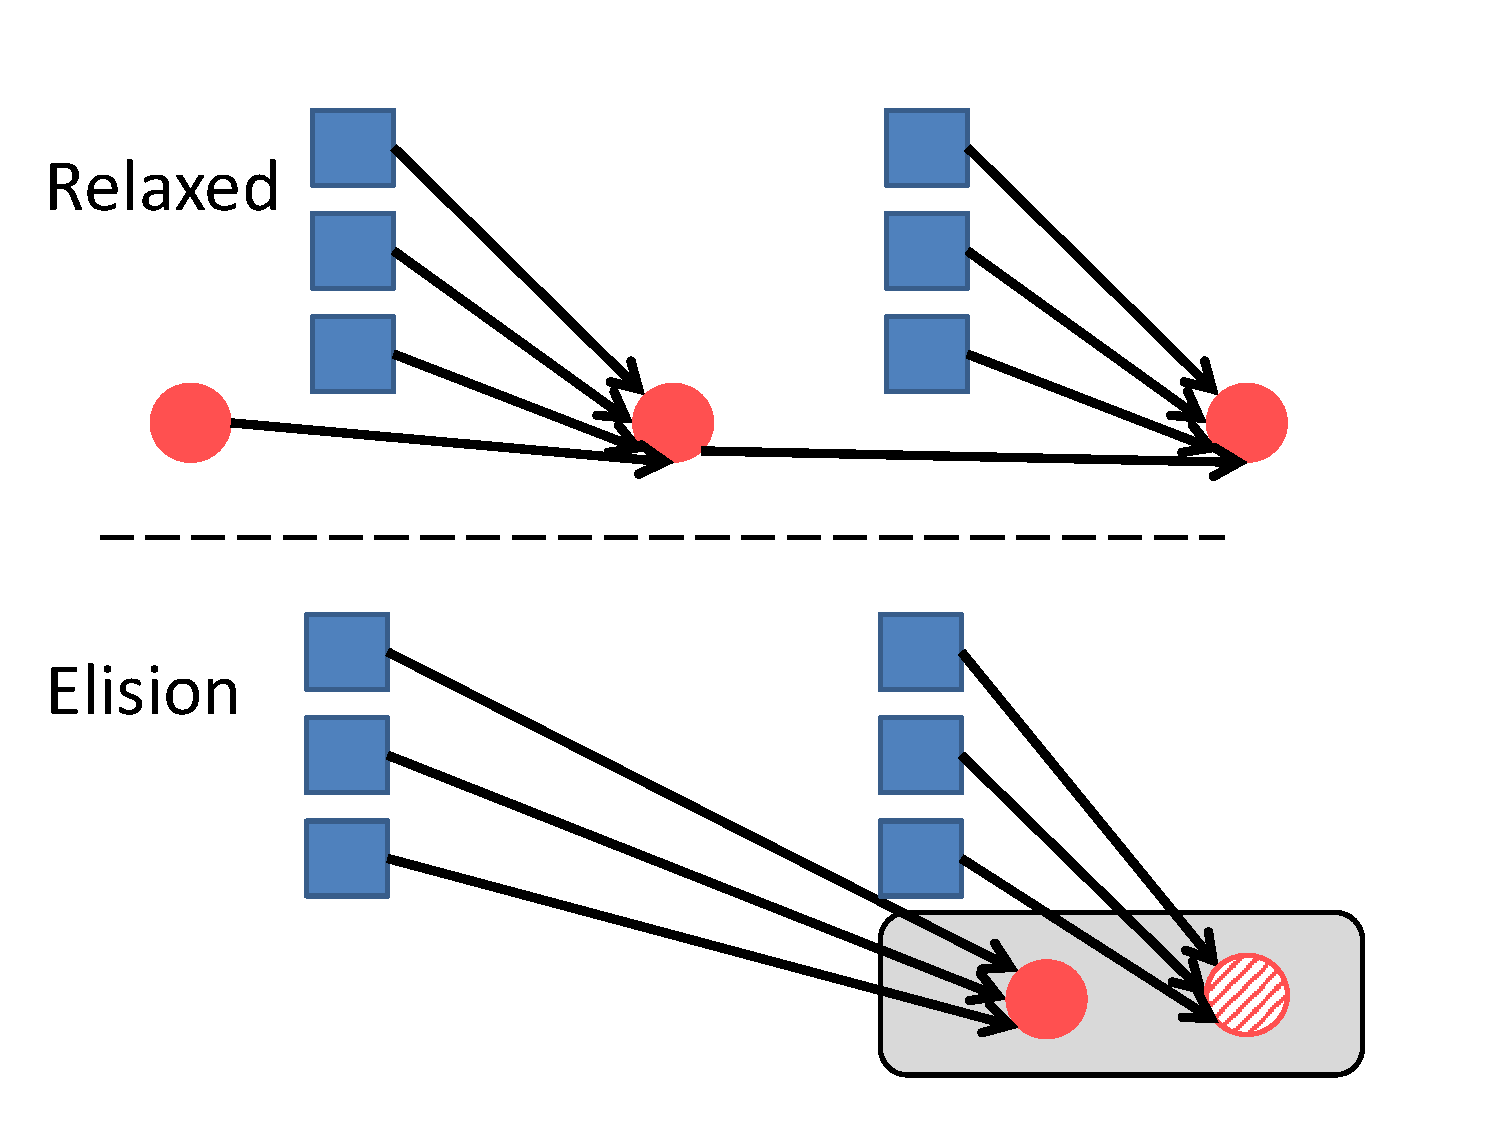
\includegraphics[width=.7\textwidth]{PMC_patterns/buffer_relaxed_elision.pdf}
\caption{\textbf{Buffer execution under relaxed persistent consistency.}  Relaxing persistent consistency removes unnecessary cross-thread dependencies (as in LPO), allows epochs to persist in parallel (as in PEO), and removes unnecessary serial epoch dependencies within threads (top).  Epochs/dependencies are elided by persisting only select counter values (bottom).}
\label{fig:buffer_relaxed_elision}
\end{figure}


\section{persistent linked list}
\label{sec:PMC_patterns:LinkedList}

\begin{figure}
\centering
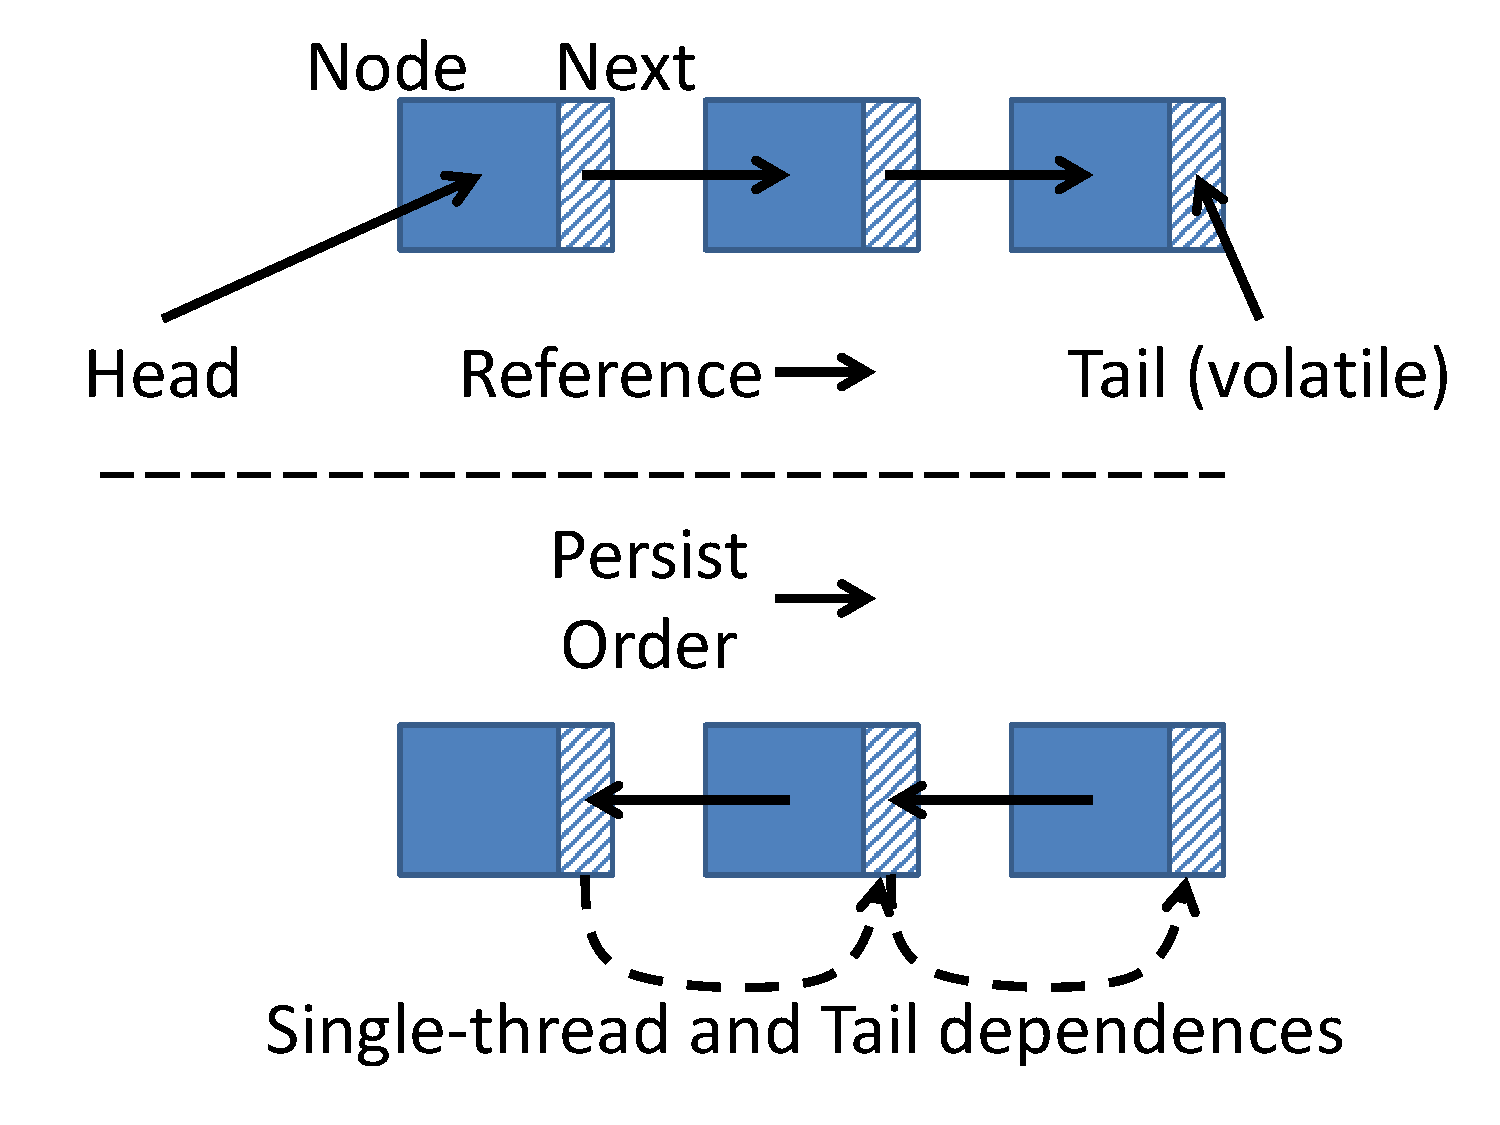
\includegraphics[width=.7\textwidth]{PMC_patterns/linkedlist.pdf}
\caption{\textbf{Persistent linked list.}  The linked list constains nonvolatile Head pointer, volatile Tail pointer, and nodes (data -- solid square; \emph{next} reference -- patterned box).  Nodes persist in parallel (data must still persist before references).  Dashed lines show unnecessary dependencies enforced by strict persistent consistency models, forming a dependence chain.  The valid list is determined at recovery by traversing from Head to the last valid node reference.  Implementing efficient sync remains a challenging.}
\label{fig:LinkedList}
\end{figure}

